\documentclass[11pt]{article}
\bibliographystyle{plain}
\usepackage{geometry} % see geometry.pdf on how to lay out the page. There's lots.
\usepackage{amsmath,amssymb} 
\usepackage{epsfig,epsf,subfigure}
\geometry{a4paper} 


%\documentclass{article}

\begin{document}
 
\LARGE
\begin{center}
TMA4280: Introduction to Supercomputing
\end{center}
\vspace{1in}

\begin{center}
{\bf Computer Architecture: \\ Single Processor Systems}
\end{center}

\Large
\vspace{0.5in}
\begin{center}
January 15, 2009
\end{center}

\vspace{0.5in}

\begin{center}
\copyright Einar M. R{\o}nquist \\
Department of Mathematical Sciences\\
NTNU, N-7491 Trondheim, Norway\\
All rights reserved
\end{center}

\large

\newpage

\section{A prototypical processor and a simple example}

We start by explaining some of the basic tasks performed by a single processor. 
The comments are particularly relevant for the MIPS R14000 processor 
used in the previous supercomputer at NTNU
(called \texttt{gridur}, a SGI Origin 3000 system used in the period 2001-2007). 
The MIPS processor is an example of a processor implementing a 
RISC architecture
(RISC - {\em Reduced Instruction Set Computer}), 
which has been a very important 
processor design over the past couple of decades. 
We will later return to comment on the  
POWER5 processor actually used in the current supercomputer at NTNU, 
in particular, some of the key differences compared to the processor discussed 
in this section. The name POWER refers to {\em Performance Optimization 
With Enhanced RISC}, and is also the name of a series of microprocessors designed 
by IBM.

\vspace{2cm}

 \begin{figure}[htbp]
  \begin{center}
    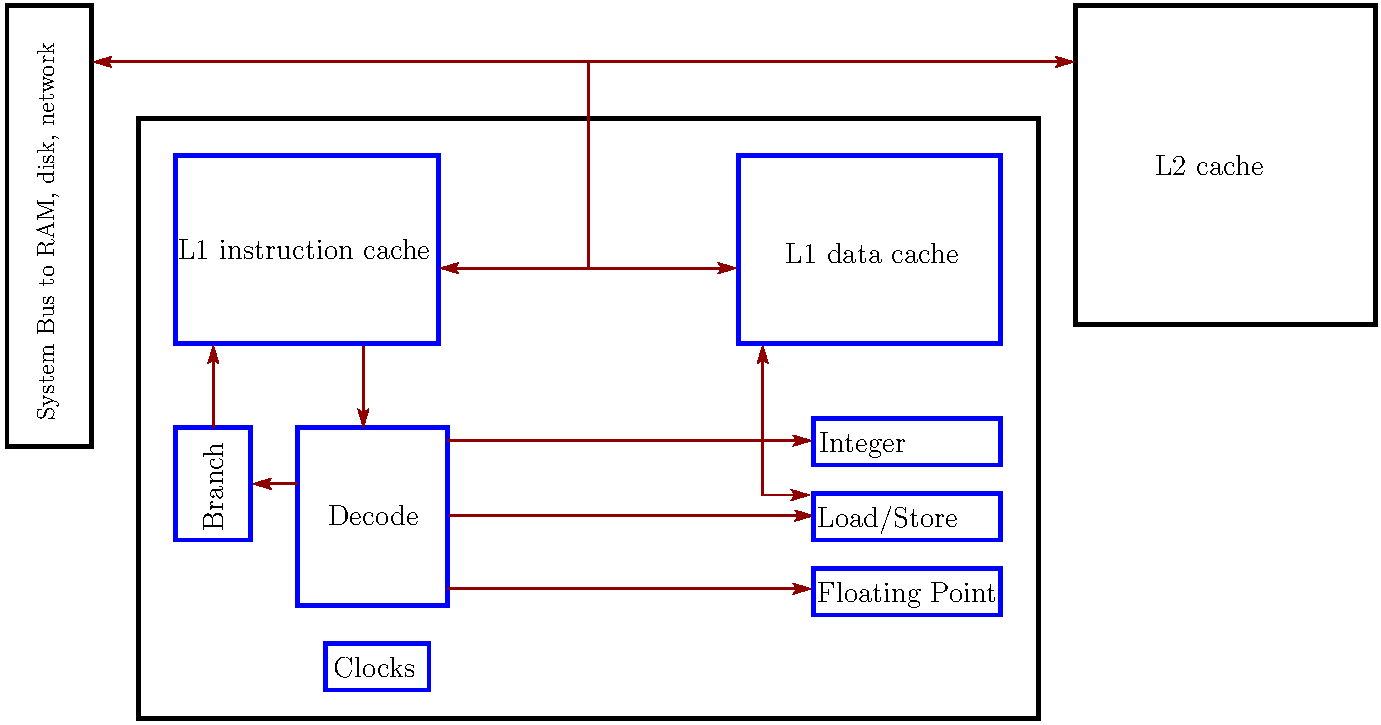
\includegraphics[scale=0.6]{Lande}
  \end{center}
  \caption{A prototypical processor, including the MIPS R14000 used in \texttt{gridur}, 
  the supercomputer at NTNU during the period 2001-2007. 
}
\label{fig:Lande}
\end{figure}

\clearpage

In order to introduce some key concepts in the RISC architecture, let us briefly 
explain what happens when we perform the following simple operation: 
\begin{align}
 c = a + b .
 \label{single:add1}
 \end{align}
 Here, we want the processor to add the two numbers $a$ and $b$ and store 
 the answer in $c$. In this case, $a$ and $b$ are referred to as operands,
 while $+$ is the operator. Hence, the simple addition of two scalars implies 
 a single floating point operation. 

The basic unit of "time" for our processor is a clock cycle. The state of the 
processor changes from  clock cycle to clock cycle, depending on what needs
to be done. Different parts/units of the processor work on different tasks
independently of each other. These tasks may correspond to different 
instructions, each in a particular phase of completion. 

Consider again the addition of two scalars.  The operation (\ref{single:add1})
may be part of a larger program involving many operations (or instructions). 
Let us assume that the instruction for the "add" operation is currently in a 
small memory module denoted as L1 cache (for instructions). 
When the execution of our program is ready to perform this operation, the 
instruction is brought into a decoder and made ready for execution. 
The addresses of the operands ($a$ and $b$) are computed and the 
operands are brought 
into two registers of the processors. We assume that the 
operands are available in the small memory module called L1 cache (for data).

The operands are then directed from the two registers 
to the floating point unit for addition (denoted as FPAdd) where 
the two numbers are added together. The whole operation takes just a few clock 
cycles. For the MIPS R14000 processor, 
this operation takes five clock cycles: 
\begin{enumerate}
\item read from register; 
\item align;
\item add; 
\item pack;
\item write to register.
\end{enumerate}

Note that the number of clock cycles required to perform this operation is
not the same as the number of bits used to store our operands 
(e.g., 64 bits in double precision). The reason is that the data flow in the 
processor happens along a "wide bus" capable of moving all the bits 
at the same time. This is an example of bit-level parallelism. 
Older processors could only move 4, 8, 16, and 32 bits at a time
and an add operation therefore took additional clock cycles to complete. 
In addition, current processors have a much higher clock frequency
(or shorter clock period) compared to older processors. 

Let us now make a few more remarks regarding the processor in Figure \ref{fig:Lande}.
We have already mentioned the floating point unit for addition, FPAdd. 
However, the processor has also other functional units. 
For example, the R14000 prosessor has five functional units 
which can operate independently from each other: 

\begin{itemize}
\item Load/Store: a unit to compute memory addresses and to bring operands to and 
from the memory; 
\item ALU1: a unit for addition and subtraction of integers, and logical operations; 
\item ALU2: a unit for addition, subtraction, multiplication, and division of integers, 
as well as logical operations; 
\item FPAdd: a unit for addition of floating point numbers; 
\item FPMult: a unit for multiplication, division, and square root of floating point numbers. 
\end{itemize}
Note that the operands used in these functional units need to come from the 
registers in the processor. If the operands are not in the registers, they have to 
be brought from the memory into the registers with a {\em load} operation. 
The answer (or output) from the functional units are also stored in registers
and subsequently stored in the memory with a {\em store} operation. 

\section{Memory hierarchy}

The example from the previous section
involving the addition of two floating point numbers 
assumed that the instruction for the operation 
(\ref{single:add1}) was in the memory module denoted as L1 cache 
for instructions; see Figure \ref{fig:Lande}.  Similarly, we assumed 
that the operands $a$ and $b$ were available in the memory module 
denoted as L1 cache for data. 

Let us now comment a bit more on what happens if these assumptions are not true.  
In this case, the program will check whether the instruction/data are 
available in the memory module denoted as L2 cache in Figure \ref{fig:Lande}.
This is a memory module which is larger than L1 cache. 
Furthermore, the L2 cache is not split into a separate module for instructions 
and a separate module for data. It also takes longer (meaning more clock cycles) 
to fetch data from L2 cache compared to L1 cache. 
It could also happen that the instruction and the data the program is looking
for is not available in L2 cache either. In this case data has to be brought 
in from main memory (RAM) or perhaps even further away (e.g. the local disk). 

Bringing instructions and data to and from memory (from cache, RAM, etc.) 
is typically a bottleneck in scientific computing. The processors are getting 
faster and faster, but the memory bandwidth (or transfer rate in bytes per second)
is not keeping up at a similar speed. Hence, for certain operations, the processor 
can become "starved" for data, meaning that it is "idle" for much 
of the time while waiting for data to be transferred to and from memory. 
The overall performance in terms of floating point operations per second 
will in such cases not be governed by the processor speed, but by the 
memory access time. 

In order to "hide" this difference in speed (i.e., processor speed versus 
memory access speed), the memory is organized in a hierarchical fashion; 
see Figure \ref{fig:MemoryHierarchy}.
\vspace{.5cm}

 \begin{figure}[htbp]
  \begin{center}
    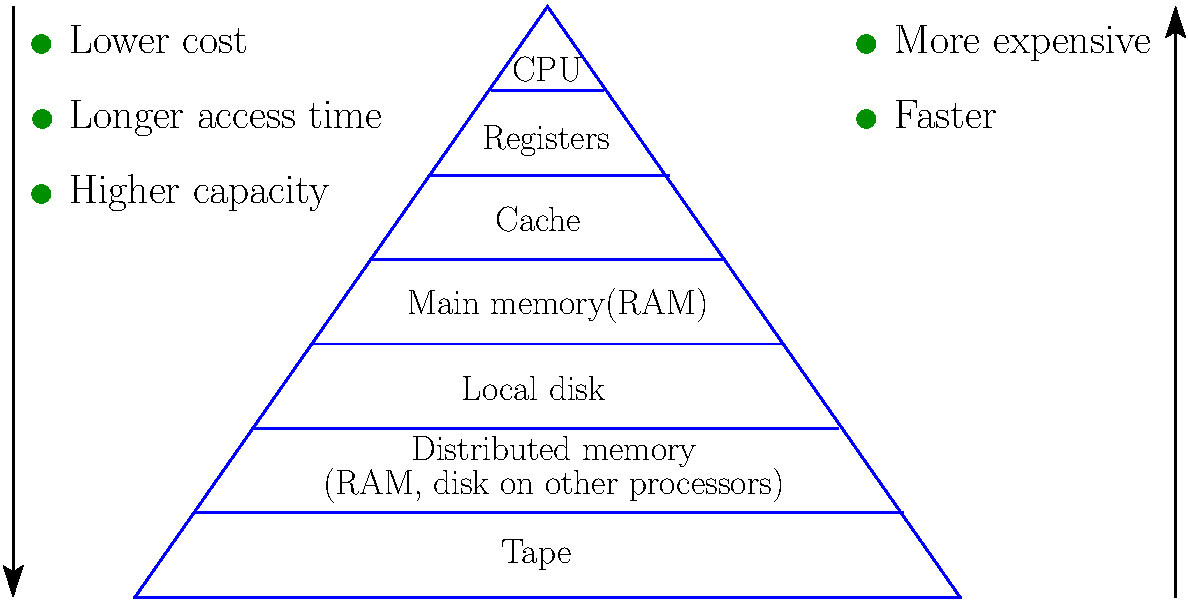
\includegraphics[scale=0.65]{MemoryHierarchy}
  \end{center}
  \caption{The memory hierarchy of a computer system. 
}
\label{fig:MemoryHierarchy}
\end{figure}
\vspace{.5cm}

The fastest part of the memory is closest to the CPU. 
For example, on the MIPS R14000, the L1 cache is on the chip. 
This part of the memory is fast, but also small because it is very expensive. 
In contrast, the main memory is much larger, but has also a much longer access time; 
see Table 1. We will later discuss in more detail how it is decided what should 
be in the L1 and L2 cache. 


%\vspace{.2in}
\begin{center}
{\bf Table 1} \\
Typical memory access times for R14000. \\
The numbers represent number of clock cycles. 
\end{center}
\begin{center}
\begin{tabular}{|c|c|c|c|c|c|c|c|} \hline
Registers & 1
  \\ \hline
L1 cache & 2-3
  \\ \hline
L2 cache & 10-12
  \\ \hline
Main memory &  100-200
  \\ \hline
Message passing & ${\cal O}(10^3)$ - ${\cal O}(10^4)$
\\ \hline
Local disk & ${\cal O}(10^6)$
  \\ \hline
\end{tabular}
\end{center}
\vspace{.2in}

We remark that message passing in Table 1 refers to communication 
between individual processors by sending messages over a network; 
we will return to a discussion of multiple processors later.


\section{Pipelining/vectorization}

Assume now that, instead of (\ref{single:add1}), we would like to add the 
two vectors $\underline{a}$ and $\underline{b}$ of length $n$
and store the result in a vector $\underline{c}$, 
i.e., 
\begin{align}
 \underline{c} = \underline{a} + \underline{b} .
 \label{single:addn}
 \end{align}
We can also write (\ref{single:addn}) as the loop
\begin{verbatim}
                          for i=1,n
                               c(i) = a(i) + b(i)
                          end
\end{verbatim}
Again, we start by assuming that the data are available in the registers.
From there, the individual vector elements $a(i)$ and $b(i)$ 
enter the floating point unit FPAdd where the numbers are added 
to produce the output elements $c(i)$, $i=1,\ldots,n$. 

We mentioned earlier that it takes five clock cycles to add two floating point 
numbers together. This would perhaps suggest that the total number of clock 
cycles for the operation (\ref{single:addn}) is $5n$, and that the total 
execution time therefore is $5n\tau$ where $\tau$ is the clock period. 
However, if things are done optimally, the total number of clock cycles 
can be reduced to approximately $n$ for $n\gg 1$. 
The reason for this is that the five stages in the adder correspond to 
independent tasks. This means that, as soon as  the addition of two 
operands (e.g., $a(i)$ and $b(i)$) has finished the first stage, 
two new operands (e.g., $a(i+1)$ and $b(i+1)$) can enter the first 
stage in the adder. Hence, after five clock cycles, the first number $c(1)$ 
in the operation (\ref{single:addn}) is ready, while the numbers
$c(2)$, $c(3)$, $c(4)$, $c(5)$, and $c(6)$ are in different phases of completion
in the adder. 

In summary, after a few clock cycles to "fill up" the adder, a new answer 
$c(i), i=2,\ldots,n$ is ready every clock cycle. This is what is refered to 
as pipelining (or sometimes vectorization). The reason behind this term is 
quite obvious: we constantly feed the floating point unit (in this case, the adder)
so that the "pipeline" is always full. In other words, we do not wait until one 
answer is ready before we start the process of adding two new numbers. 
In this way, we achieve a certain level of parallelism in the sense that 
asymptotically (for long vector lengths), the adder works simultaneously 
on five different pairs of operands. 

The above discussion assumed that the data (i.e., the operands
$a(i)$ and $b(i)$, $i=1,\ldots,n$) are ready for the adder with no delay. 
Whether this is possible or not, depends on the particular processor. 
In the case of the MIPS R14000 processor, it is not possible 
to achieve this performance. The reason is that, in the best case, 
only a single floating point number can be brought between the memory
(L1 cache) and a register at a time. Since we need to fetch two operands, 
$a(i)$ and $b(i)$, per floating point operation, and store the answer $c(i)$
back to memory, 
a minimum of three clock cycles are needed for memory transfer per addition. 
Hence, even though the floating point unit (the adder) can theoretically 
complete one addition per clock cycle, the memory traffic will be the bottleneck, 
at least for large $n$. 

The only possibility for achieving a better performance, 
is if all the operands are already available in the processors registers. 
However, since a processor only has a limited number of registers
(on the MIPS R14000, the number of registers is 64), such performance
cannot be acheived if $n\gg 1$. 

Let us now predict the optimal performance for the operation (\ref{single:addn})
in the case $n\gg 1$ on Gridur. The clock cycle for each processor is 500 MHz. 
Hence, the clock period is 2 ns. Since each floating point operation will 
asymptotically require three clock cycles due to the fetch and store operations
(see the discussion above), each floating point operation will at least require 
three clock cycles or 6 ns. Hence, the maximum performance for the operation 
(\ref{single:addn}) is $1/(6\cdot 10^{-9})$ floating point operations per second, 
or approximately 167 MFLOPS. In practice, less performance may be achieved, 
in particular, if the operands need to first be brought in from deeper layers 
of the memory hierarchy; see Figure \ref{fig:MemoryHierarchy}.

%\newpage

\section{Superscalar operations}

Consider now a modification of the operation (\ref{single:addn}) to 
the following operation:
\begin{align}
 \underline{c} = \underline{a} + \gamma\cdot \underline{b} .
 \label{single:addmultn}
 \end{align}
Here, each vector element $b(i)$, $i=1,\ldots,n$ is multiplied with a 
scalar, $\gamma$, before being added to $a(i)$. Similar to the operation
(\ref{single:addn}) the result of each addition is stored as the vector element $c(i)$. 

The new operation here is the multiplication. As mentioned earlier, 
each R14000 processor has 
a separate floating point unit for multiplication, FPMult. 
Similar to the add operation, multiplying two numbers also take five clock cycles: 
\begin{enumerate}
\item read from register; 
\item multiply;
\item sum product; 
\item pack;
\item write to register.
\end{enumerate}
Hence, all the comments made in the previous section 
for the operation (\ref{single:addn}) also apply if the add operation $+$ is 
replaced by multiplication $*$. 

Let us now comment on what happens when we combine both 
multiplication and addition as in (\ref{single:addmultn}). 
Again, let us first assume that all the data are readily available 
(e.g., stored in the registers). The vector elements 
$b(i)$ are brought to the multiplier where each element is multiplied 
by the scalar $\gamma$; see Figure \ref{fig:SuperScalar}. 
After a startup time of five clock cycles, a new answer is coming out 
from the multiplier every clock cycle. We assume here that the 
pipelining feature is exploited. 
\vspace{.5cm}

\begin{figure}[htbp]
  \begin{center}
    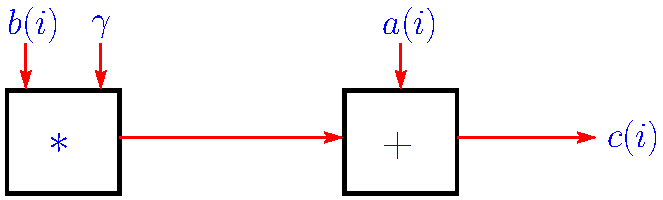
\includegraphics[scale=0.9]{SuperScalar}
  \end{center}
  \caption{The superscalar operation multiply and add. 
}
\label{fig:SuperScalar}
\end{figure}
\vspace{.5cm}

Each output from the multiplier is now channeled directly as an input 
to the adder where it is added to the vector element $a(i)$. 
After another five clock cycles, the answer $c(i)$ is ready. 
Hence, after a startup time of 10 clock cycles 
(5 for the multiplier and 5 for the adder), we get one complete 
answer $c(i), i=1,\ldots,n$ as output every clock cycle. 
Asymptotically (i.e., for large vector lengths), the theoretical performance 
is therefore two floating point operations per clock cycle. 
This way of piping the output from one floating point unit into 
the input for another unit is denoted as {\em superscalar} capability. 
Similar to the pipelining feature of the adder and the multiplier, 
the superscalar capability offers yet another possibility of parallelism
in the sense that each single processor is capable of performing 
addition and multiplication at the same time (for sufficiently long vector lengths). 

In practice, the processor has only a limited number of registers, 
and we need to fetch the operands from memory (L1 cache) 
and store the answers in memory.  
Similar to the operation (\ref{single:addn}), each complete 
vector element $c(i)$ will require three clock cycles due to the 
memory traffic. However, in contrast to the operation (\ref{single:addn}),
the operation (\ref{single:addmultn}) implies two floating point operations
instead of one for each complete vector element $c(i)$. 
The maximum single-process performance we can obtain 
on R14000 for (\ref{single:addmultn}) is thus 
twice the performance for (\ref{single:addn}), i.e., 333 MFLOPS. 

\section{Cache}

Let us now discuss in more detail the interaction between the 
cache and the main memory. The main purpose of the cache is to 
keep copies of data in extra (and fast) memory close to the CPU in order to "hide"
the relatively slow transfer rate between the main memory and the processor. 

Because fast caches are expensive, they tend to be small. 
As an example, we give the memory sizes for the R14000 processors. 
On \texttt{gridur}, four individual processors shared up to 4 Gbytes of main memory. 
Each processor had an L2 cache of size 8 Mbytes and two L1 caches 
(one for instructions and one for data), each only of size 32 Kbytes. 
Hence, the L1 cache for data can only hold up to 4000 floating point numbers
(assuming double precision), 
which is relatively small in the context of simulating systems with thousands or  
millions of unknowns (e.g., for the numerical solution of partial differential equations). 
The L2 cache can hold more data, but the transfer rate is a little bit longer 
compared to the L1 cache; see Table 1. 

The cache is smaller than the main memory by some power of 2. 
Hence, a strategy for mapping memory locations to cache locations needs to be defined. 
One strategy is to use what is refered to as a {\em direct mapped cache}. 
In this case, each location in main memory corresponds to a unique location in cache; 
see Figure \ref{fig:DirectMappedCache}. The main memory address is split into two parts: the first bits of the memory address are called the {\em set bits} and these bits 
give the precise cache address.  
The remaining bits are called the {\em tag bits}, 
and these are used to determine if a copy of the content 
at the particular main memory location has been copied into the cache location 
given by the set bits. With this strategy we see that several main  
memory addresses map to the same cache address. 


\begin{figure}[htbp]
  \begin{center}
    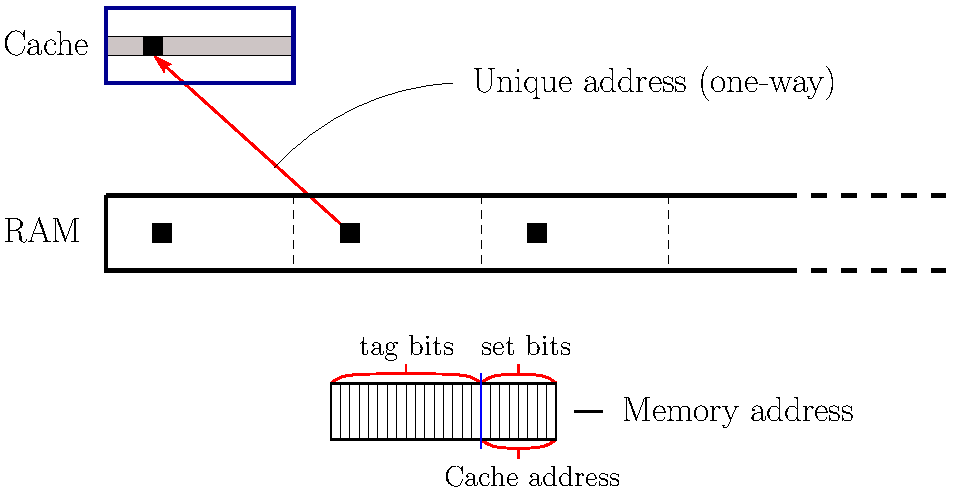
\includegraphics[scale=0.85]{DirectMappedCache}
  \end{center}
  \caption{A direct mapped cache. 
}
\label{fig:DirectMappedCache}
\end{figure}

When some particular data is requested by the program, e.g., a floating point number,
the processor will check whether the data is stored in L1 cache. 
If it is not in L1 cache, the processor will check whether the data is stored in 
L2 cache. If this is the case, the requested data will be copied from the L2 cache 
into L1 cache. If the data is not in L2 cache either, the data will have to be brought 
in from main memory. In this case, a copy will be made in L2 cache as well as 
in L1 cache. 

Note that, when a floating point number (or an integer) is requested by 
the program, more than a single number is copied into cache. 
The minimum amount of data copied is called a {\em cache line}. 
For the R14000 processor, the cache line for the L1 cache is 32 bytes
(corresponding to four floating point numbers in double precision), 
while the cache line for the L2 cache is 128 bytes 
(corresponding to 16 floating point numbers in double precision). 
The extra numbers copied are the numbers in the adjacent memory 
locations in main memory.  

Consider again the operation (\ref{single:addn}). Assume that the 
vectors $\underline{a}$, $\underline{b}$ and $\underline{c}$ represent 
floating point numbers in double precision, and that the vectors are 
stored after each other in main memory. Let the vector length $n=4000$, 
i.e., each vector will precisely fill the L1 data cache. 
For every element $c(i)$ computed, the operands $a(i)$ and $b(i)$ 
will need to be brought in all the way from main memory due to the fact 
that $a(i)$, $b(i)$ and $c(i)$ happen to have the same cache address. 
A severe drop in performance will be observed in this case. 
This situation is refered to as cache trashing; see Figure \ref{fig:CacheTrashing}.
\vspace{.5cm}

\begin{figure}[htbp]
  \begin{center}
    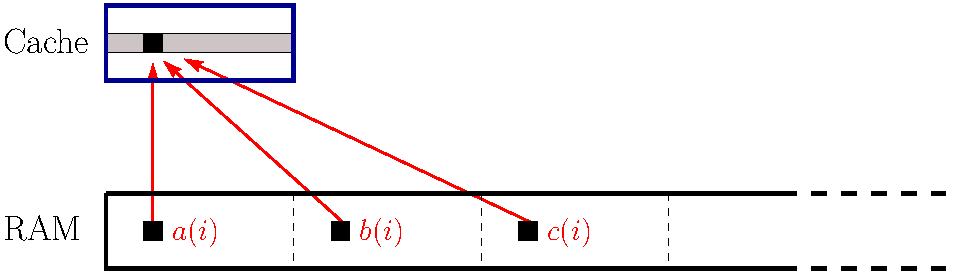
\includegraphics[scale=0.85]{CacheTrashing}
  \end{center}
  \caption{Cache trashing. 
}
\label{fig:CacheTrashing}
\end{figure}

\newpage
Cache trashing can for example be avoided by storing the elements in the 
vectors $\underline{a}$, $\underline{b}$ and $\underline{c}$ in a different way; 
see Figure \ref{fig:AdjacentMemory}. We remark that the crash trashing 
example given here is perhaps not likely to happen. Nonetheless, 
it illustrates the point that severe performance degradation is possible to 
observe  due to undesirable memory traffic. 
\vspace{.5cm}

\begin{figure}[htbp]
  \begin{center}
    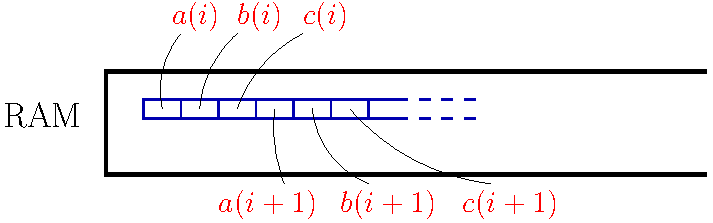
\includegraphics[scale=0.9]{AdjacentMemory}
  \end{center}
  \caption{Adjacent memory. 
}
\label{fig:AdjacentMemory}
\end{figure}
\vspace{.5cm}

Finally, we mention an alternative strategy for mapping memory locations 
to cache locations, namely, $n$-way set-associative cache; 
see Figure \ref{fig:NWayCache}.
Here, there are $n$ "ways" to map a memory address to a cache address, 
i.e., a particular memory location can potentially end up in one of $n$ cache lines. 
The particular cache line chosen depends on the replacement policy: 
\begin{itemize}
\item Least Recently Used (LRU);
\item Least Frequently Used (LFU);
\item Random. 
\end{itemize}

In the context of numerical solution of partial differential equations, 
the alternative LRU generally gives the best performance. 
This can be understood by the fact that such problems typically 
exhibit significant locality in time and space: data that has recently 
been used has a high chance of being used again in the near future; 
and data close (in space) to recently used data has a high chance of 
being used in the near future. 
\vspace{2cm}

\begin{figure}[htbp]
  \begin{center}
    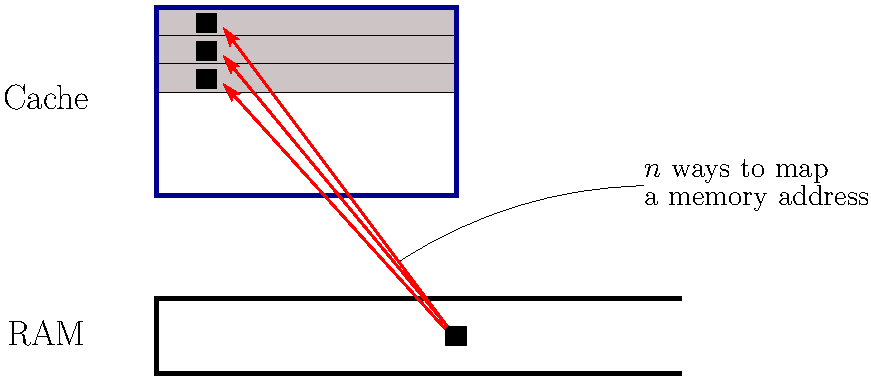
\includegraphics[scale=0.8]{NWayCache}
  \end{center}
  \caption{$n$-way set-associative cache. 
}
\label{fig:NWayCache}
\end{figure}


\begin{thebibliography}{99}

\bibitem {} D.E. Culler and J.P. Singh, Parallel Computer Architecture, 
{\em Morgan Kaufmann Publishers, Inc.}, 1999. 

\bibitem {} C.C. Douglas, G. Haase, J. Hu, M. Kowarschik, U. Rude, 
and C. Weiss, Portable memory hierarchy techniques for PDE solvers: Part I, 
{\em SIAM News}, Vol. 33, No. 5, 2000. 

\bibitem  {} B. Lande, Optimalisering av flyttallsintensive programmer, 
Institutt for matematiske fag, NTNU, 2004. (In Norwegian.)


\end{thebibliography}

\end{document}


\begin{figure}[htbp]
  \begin{center}
    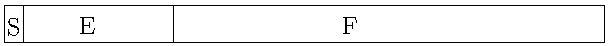
\includegraphics[scale=1]{ieee}
  \end{center}
  \caption{Each floating point has a binary representation with 
three fields: $S$ denotes the sign of the number, 
$E$ is an exponent, and $F$ is the fraction part of the mantissa.
}
\label{fig:fp}
\end{figure}


\begin{center}
{\bf Table 1} \\
Number of bits for common floating point precisions
\end{center}
\begin{center}
\begin{tabular}{|c|c|c|c|c|c|c|c|} \hline
Precision & $S$ & $E$ & $F$ & Total  
  \\ \hline
Single & $1$ & $8$ & $23$ & 32  
  \\ \hline
Double & $1$ & $11$ & $52$ & 64 
  \\ \hline
\end{tabular}
\end{center}


\vspace{.2in}
\noindent {\bf Exercise 1}. Consider the maximum and minimum numbers 
derived in (\ref{maxnumber})-(\ref{minnumber}). How many digits should we include in each
of these numbers?\\
\\
\noindent {\bf Exercise 2}. Find the binary floating point
representation of the decimal number 4.25 in single precision.\\
\\
\noindent {\bf Exercise 3}. How many digits of accuracy does a 
floating point number in double precision have? 




